\documentclass[14pt]{extbook}
\usepackage{multicol, enumerate, enumitem, hyperref, color, soul, setspace, parskip, fancyhdr} %General Packages
\usepackage{amssymb, amsthm, amsmath, latexsym, units, mathtools} %Math Packages
\everymath{\displaystyle} %All math in Display Style
% Packages with additional options
\usepackage[headsep=0.5cm,headheight=12pt, left=1 in,right= 1 in,top= 1 in,bottom= 1 in]{geometry}
\usepackage[usenames,dvipsnames]{xcolor}
\usepackage{dashrule}  % Package to use the command below to create lines between items
\newcommand{\litem}[1]{\item#1\hspace*{-1cm}\rule{\textwidth}{0.4pt}}
\pagestyle{fancy}
\lhead{Makeup Progress Quiz 3}
\chead{}
\rhead{Version B}
\lfoot{1648-1753}
\cfoot{}
\rfoot{Summer C 2021}
\begin{document}

\begin{enumerate}
\litem{
Choose the equation of the function graphed below.
\begin{center}
    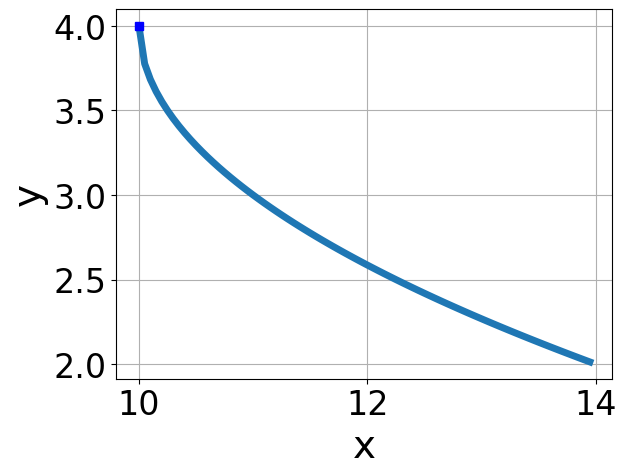
\includegraphics[width=0.5\textwidth]{../Figures/radicalGraphToEquationB.png}
\end{center}
\begin{enumerate}[label=\Alph*.]
\item \( f(x) = - \sqrt[3]{x - 10} + 4 \)
\item \( f(x) = \sqrt[3]{x - 10} + 4 \)
\item \( f(x) = \sqrt[3]{x + 10} + 4 \)
\item \( f(x) = - \sqrt[3]{x + 10} + 4 \)
\item \( \text{None of the above} \)

\end{enumerate} }
\litem{
Choose the graph of the equation below.\[ f(x) = \sqrt[3]{x - 10} + 6 \]\begin{enumerate}[label=\Alph*.]
\begin{multicols}{2}\item 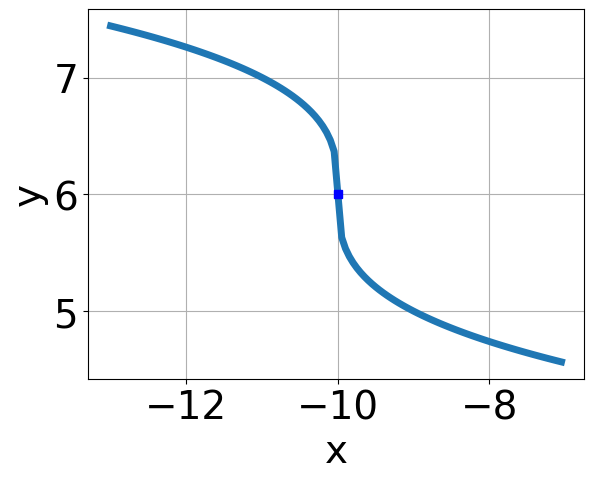
\includegraphics[width = 0.3\textwidth]{../Figures/radicalEquationToGraphCopyAB.png}\item 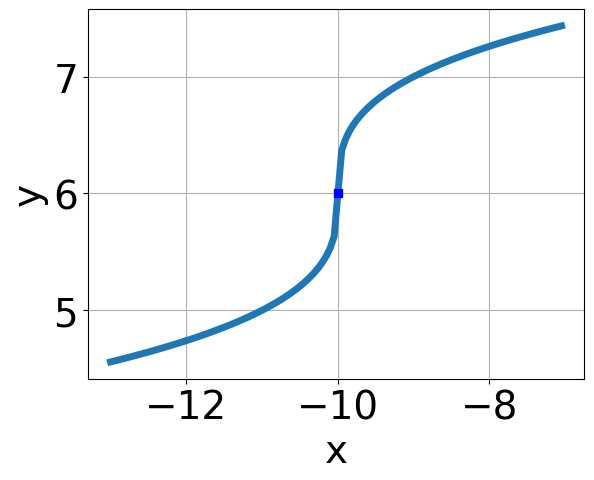
\includegraphics[width = 0.3\textwidth]{../Figures/radicalEquationToGraphCopyBB.png}\item 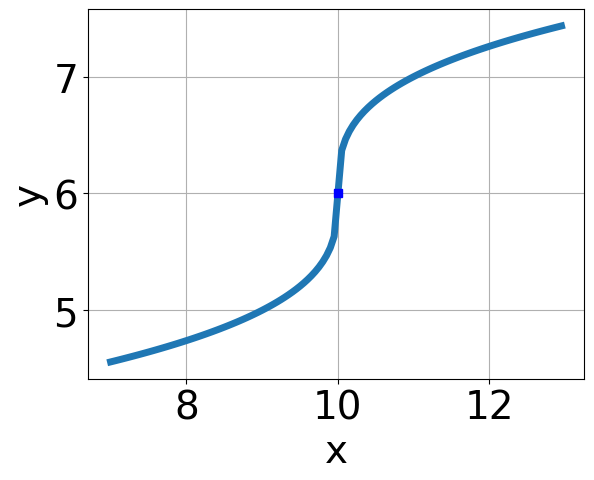
\includegraphics[width = 0.3\textwidth]{../Figures/radicalEquationToGraphCopyCB.png}\item 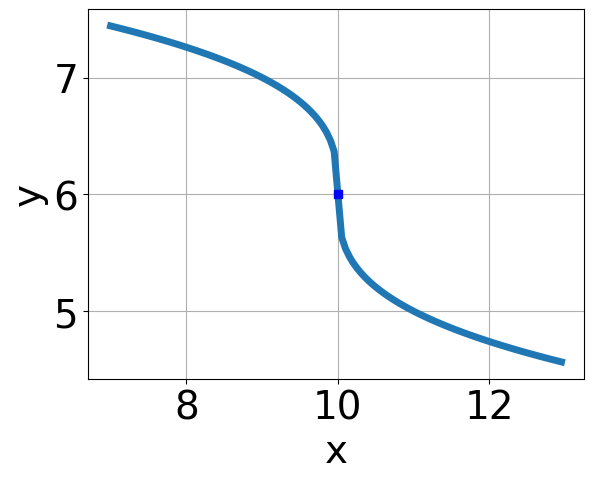
\includegraphics[width = 0.3\textwidth]{../Figures/radicalEquationToGraphCopyDB.png}\end{multicols}\item None of the above.
\end{enumerate} }
\litem{
What is the domain of the function below?\[ f(x) = \sqrt[6]{5 x + 9} \]\begin{enumerate}[label=\Alph*.]
\item \( (-\infty, \infty) \)
\item \( (-\infty, a], \text{where } a \in [-4.5, -0.8] \)
\item \( (-\infty, a], \text{where } a \in [-0.7, 0.6] \)
\item \( [a, \infty), \text{ where } a \in [-3.04, -0.59] \)
\item \( [a, \infty), \text{where } a \in [-1.36, 0.62] \)

\end{enumerate} }
\litem{
Solve the radical equation below. Then, choose the interval(s) that the solution(s) belongs to.\[ \sqrt{32 x^2 + 24} - \sqrt{-76 x} = 0 \]\begin{enumerate}[label=\Alph*.]
\item \( x \in [-1.81,-0.27] \)
\item \( x_1 \in [-0.14, 0.63] \text{ and } x_2 \in [0.4,3.9] \)
\item \( x_1 \in [-2.1, -1.51] \text{ and } x_2 \in [-1.1,0.2] \)
\item \( x \in [-2.1,-1.51] \)
\item \( \text{All solutions lead to invalid or complex values in the equation.} \)

\end{enumerate} }
\litem{
Choose the equation of the function graphed below.
\begin{center}
    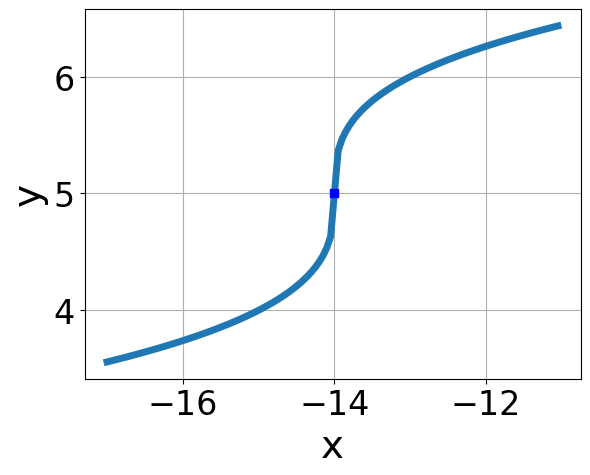
\includegraphics[width=0.5\textwidth]{../Figures/radicalGraphToEquationCopyB.png}
\end{center}
\begin{enumerate}[label=\Alph*.]
\item \( f(x) = \sqrt{x + 14} + 5 \)
\item \( f(x) = - \sqrt{x - 14} + 5 \)
\item \( f(x) = - \sqrt{x + 14} + 5 \)
\item \( f(x) = \sqrt{x - 14} + 5 \)
\item \( \text{None of the above} \)

\end{enumerate} }
\litem{
Solve the radical equation below. Then, choose the interval(s) that the solution(s) belongs to.\[ \sqrt{-6 x - 7} - \sqrt{-3 x + 7} = 0 \]\begin{enumerate}[label=\Alph*.]
\item \( x_1 \in [-4.17, -0.17] \text{ and } x_2 \in [2.33,5.33] \)
\item \( x \in [-0,1] \)
\item \( x \in [-5.67,-1.67] \)
\item \( x_1 \in [-5.67, -1.67] \text{ and } x_2 \in [-1.17,1.83] \)
\item \( \text{All solutions lead to invalid or complex values in the equation.} \)

\end{enumerate} }
\litem{
Solve the radical equation below. Then, choose the interval(s) that the solution(s) belongs to.\[ \sqrt{-48 x^2 - 9} - \sqrt{-42 x} = 0 \]\begin{enumerate}[label=\Alph*.]
\item \( x \in [0.46,0.53] \)
\item \( x_1 \in [0.36, 0.41] \text{ and } x_2 \in [-0.38,1.8] \)
\item \( \text{All solutions lead to invalid or complex values in the equation.} \)
\item \( x \in [0.36,0.41] \)
\item \( x_1 \in [-0.55, -0.35] \text{ and } x_2 \in [-1.34,-0.02] \)

\end{enumerate} }
\litem{
Solve the radical equation below. Then, choose the interval(s) that the solution(s) belongs to.\[ \sqrt{-8 x - 6} - \sqrt{7 x - 7} = 0 \]\begin{enumerate}[label=\Alph*.]
\item \( x_1 \in [-0.78, -0.75] \text{ and } x_2 \in [0.83,1.87] \)
\item \( x \in [-0.93,-0.76] \)
\item \( \text{All solutions lead to invalid or complex values in the equation.} \)
\item \( x \in [0.01,0.41] \)
\item \( x_1 \in [-0.78, -0.75] \text{ and } x_2 \in [-0.84,0.73] \)

\end{enumerate} }
\litem{
Choose the graph of the equation below.\[ f(x) = \sqrt{x + 14} - 6 \]\begin{enumerate}[label=\Alph*.]
\begin{multicols}{2}\item 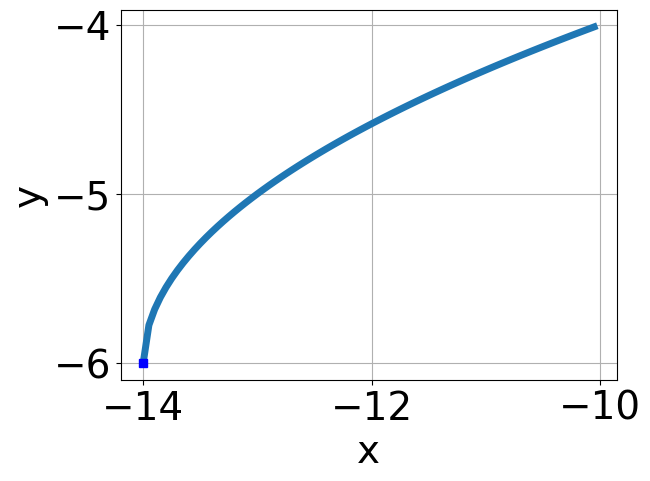
\includegraphics[width = 0.3\textwidth]{../Figures/radicalEquationToGraphAB.png}\item 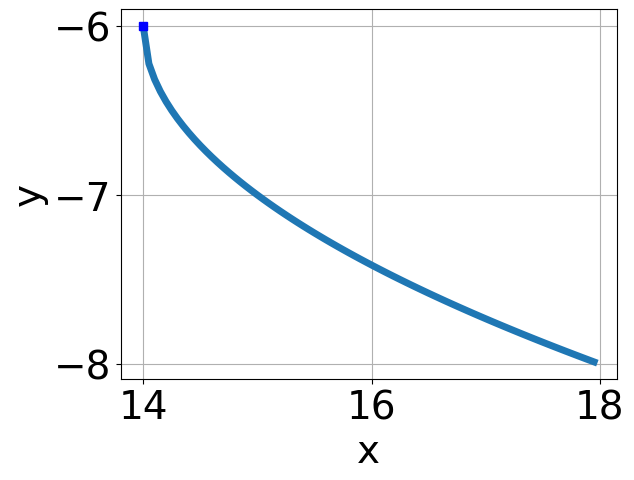
\includegraphics[width = 0.3\textwidth]{../Figures/radicalEquationToGraphBB.png}\item 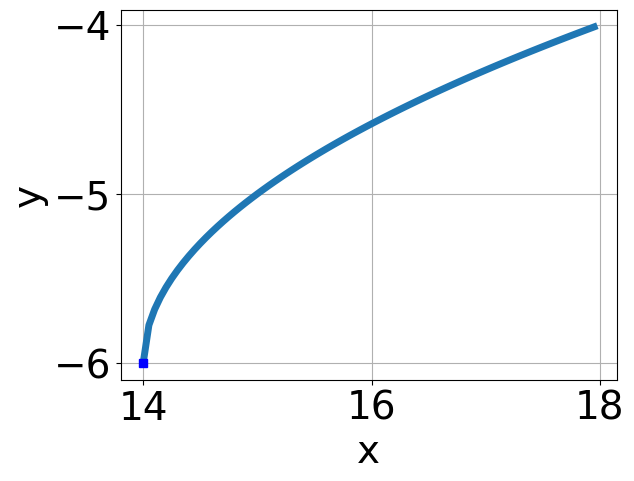
\includegraphics[width = 0.3\textwidth]{../Figures/radicalEquationToGraphCB.png}\item 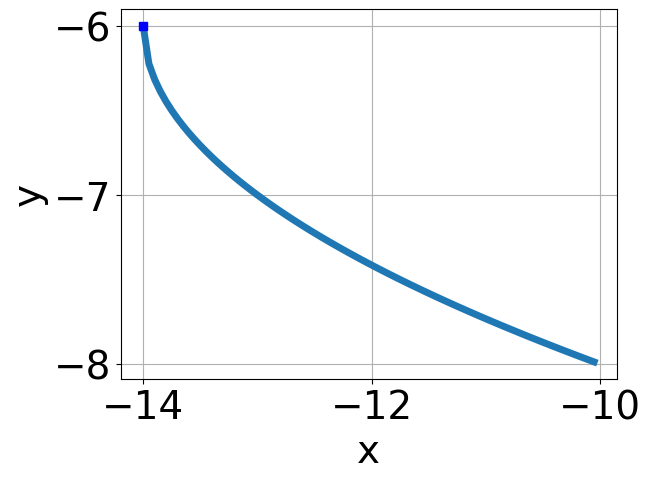
\includegraphics[width = 0.3\textwidth]{../Figures/radicalEquationToGraphDB.png}\end{multicols}\item None of the above.
\end{enumerate} }
\litem{
What is the domain of the function below?\[ f(x) = \sqrt[3]{5 x - 7} \]\begin{enumerate}[label=\Alph*.]
\item \( (-\infty, \infty) \)
\item \( \text{The domain is } (-\infty, a], \text{   where } a \in [0.5, 0.95] \)
\item \( \text{The domain is } (-\infty, a], \text{   where } a \in [1.23, 2.47] \)
\item \( \text{The domain is } [a, \infty), \text{   where } a \in [-0.9, 1.1] \)
\item \( \text{The domain is } [a, \infty), \text{   where } a \in [0.9, 2.8] \)

\end{enumerate} }
\end{enumerate}

\end{document}